
\documentclass[journal]{IEEEtran}
%\usepackage[UTF8]{ctex}
\usepackage{graphicx}
\usepackage{algorithm}
\usepackage{algpseudocode}

\renewcommand{\algorithmicrequire}{ \textbf{Input:}}
\renewcommand{\algorithmicensure}{ \textbf{Output:}}

\begin{document}

hello world

this is my first fig \ref{test-figure}
%214712283曹泽群

\cite{CZQ-cite1}

\begin{table}
\centering
\caption{test table}
\begin{tabular}{|p{5.1em}|p{5.1em}|r|}
\hline
name & class & id \\
\hline
czq & 21 & 214712283 \\
\hline
\end{tabular}
\end{table}

\begin{figure}
\centering
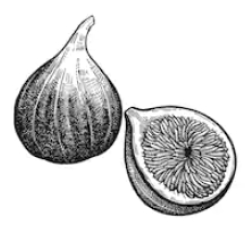
\includegraphics[width=6.5cm]{fig1.png}

\caption{test figure}
\label{test-figure}
\end{figure}

\begin{algorithm}[t]
\caption{algorithm caption} %算法的名字
\hspace*{0.02in} {\bf Input:} %算法的输入, \hspace*{0.02in}用来控制位置,同时利用 \\ 进行换行
input parameters A, B, C\\
\hspace*{0.02in} {\bf Output:} %算法的结果输出
output result
\begin{algorithmic}[1]
\State some description % \State 后写一般语句
\For{condition} % For 语句,需要和EndFor对应
  \State ...
  \If{condition} % If 语句,需要和EndIf对应
    \State ...
  \Else
    \State ...
  \EndIf
\EndFor
\While{condition} % While语句,需要和EndWhile对应
  \State ...
\EndWhile
\State \Return result
\end{algorithmic}
\end{algorithm}



\bibliographystyle{IEEEtran}
\bibliography{214712283czq}
\nocite{CZQ-cite1}
\nocite{CZQ-cite2}
\end{document}